\section{Methodology}
\label{sec:metho}
In this section, we begin by formulating the problem. 
%
And then we put forward our main methods.
%
Fig.~\ref{fig:Pipeline} shows the diagram of our proposed method.
%
First, propageting the labels from the labeled frames to their adjacent frames to generate pseudo ground truth.
Then we train a segmentation network with both the manually labeled frames and frames with pseudo labels, as well as a self-supervised loss function to ensure the temporal consistency between adjacent frames.
\begin{comment}
In a set of video sequences of which only a few frames are manually labeled with pixel-wise semantic labels, we first propagate the labels from the labeled frames to their adjacent frames to generate pseudo ground truth. 
Then we train a segmentation network with both the manually labeled frames and frames with pseudo labels, as well as a loss function to ensure the temporal consistency between adjacent frames.
\end{comment}
\subsection{Problem formulation}
In a set of video sequences $X := (x_1,...,x_m,x_{m+1},...,x_n)$ of which only a few frames $X_M := (x_1,...,x_m)$ are manually labeled with pixel-wise semantic labels $Y_M := (y_1,...,y_m)$. 
%
The remaining frames $X_U := (x_{m+1},...,x_n)$ are unlabeled.
%
The goal in our semi-supervised learning is to use both labeled frames and part of unlabeled frames to train a semantic segmentation network that provides the prediction of unseen frames.

\subsection{Pseudo Ground Truth Generation}
%
In a video sequence of which one frame $F_t$ is manually annotated with pixel-wise semantic labels $G_t$, we propagate these labels to its adjacent $2K$ frames $\mathcal{F}=\{F_{t-K},\ldots, F_{t+K}\}$ via two steps.
%
First, for each frame $F_k$ in $\mathcal{F}$, a homography matrix $\mathbf{H}_{tk}$ is first computed by looking for matched SIFT keypoints with RANSAC verification.
%
In order to avoid large distortion or content changes, we only keep the video frames whose transformation matrix to the reference frame $F_t$
% 
\begin{equation}
\centering
\begin{aligned}
\mathbf{H}_{tk}
=
\left[
\begin{array}{ccc}
h_{00} & h_{01} & h_{02}\\
h_{10} & h_{11} & h_{12}\\
h_{20} & h_{21} & 1\\
\end{array}
\right] \\
s.t. \hspace{0.2cm}0.95<\max{\left\{\left|h_{00}\right|,\left|h_{01}\right|,\left|h_{10}\right|,\left|h_{11}\right|\right\}}&<1.05,\\
\max{\left\{\left|h_{02}\right|,\left|h_{12}\right|,\left|h_{20}\right|,\left|h_{21}\right|\right\}}&<15.\\
\end{aligned}
\end{equation}


Fig.~\ref{fig:PGT} shows an example of the generated pseudo ground truth labels from a reference frame $F_t$. 
It can be seen that most of the semantic labels are well propagated and can be used as extra data for network training. 
% 
However, there are still some noisy labels in the propagated PGT, especially at the object boundary regions. 
%
Therefore, we add a manual filtering process to remove the frames where there are obvious visual artifacts in the generated pseudo labels.

A toy example showing the results of label propagetion by our method, rigid body transformation and flow estimation is shown in Fig.~\ref{fig:PGT_Com}.
%
Compared to other PGT generated methods, our approach keeps the boundary of PGT better.

\begin{figure}[t]
	\centering
	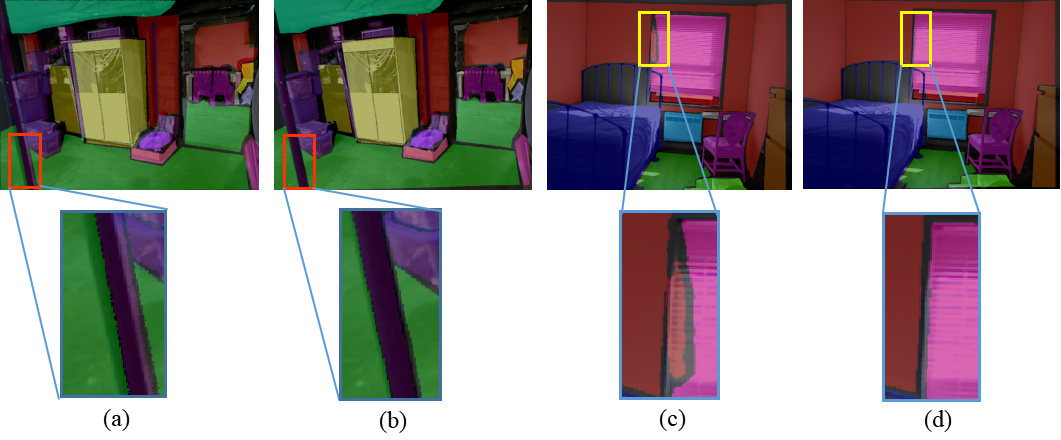
\includegraphics[width=\columnwidth]{figure/PGT_compared.png}
	%	\vspace*{-0.6cm} 
	\caption{Comparison of different methods of annotation propagetion. (a) PGT generated by rigid body transformation. The camera external parameters is evaluated by Bundler and the depth is filled using NYU-v2 official code. (b)(d) PGT of our method. (c) PGT generated by optical flow using PWC-Net\cite{Sun2018}.}
	\label{fig:PGT_Com}
	%	\vspace*{-0.35cm} 
\end{figure}

%\noindent\textbf{Training Segmentation Network using Temporal Consistency.}
\subsection{Training Segmentation Network using Temporal Consistency}
%
As Fig.~\ref{fig:Pipeline} shows, we train a semantic segmentation network using two adjacent frames in a video instead of using a single labeled frame.  
% 
First, two adjacent frames $F_{t-1}$ and $F_t$ are passed through a basic segmentation network to predict semantic labels $S_{t-1}$ and $S_{t}$.
%
The basic segmentation network could be any existing network for semantic segmentation. 
We use RDFNet\cite{Park2017}, which is a high-precision network for semantic segmentation of a RGBD image.
% The input of RDFNet is a RGBD image. 
%The depthmap is encoded into a 3D image called HHA \cite{Gupta2014} which encodes {\bf H}eight above ground and {\bf H}orizontal disparity in addition to the {\bf A}ngle with gravity for each pixel .
%Four multi-model feature fusions (MMF) are used to fully exploit multi-level HHA and RGB images' features.
% And then four RefineNet blocks are applied to refine the output of MMF gradually.
% More details of RDFNet could be found in \cite{Park2017}. 



Second, the predicted semantic score map $S_{t-1}$ for frame $F_{t-1}$ is warped to $\hat{S}_{t}$ according to the optical flow $O_{t-1,t}$ between $F_t$ and $F_{t-1}$, which is estimated using an efficient and accurate model PWC-Net~\cite{Sun2018} from two frames. 
We implement a bilinear interpolation for $40$ dimensional score vector of each pixel in $S_{t-1}$, where 40 is the total number of object classes in the dataset. 
\begin{equation}
\centering
\hat{S}_{t}=Warp(S_{t-1},O_{t-1,t}).
\end{equation}
%
An argmax layer is then added on the warped score map ${\hat{S}_{t}}$ to generate the warped semantic prediction $W_{t}$.
\begin{comment}
\begin{equation}
\centering
W_{t}=\arg \max \hat{S}_{t-1}.
\end{equation}
\end{comment}


Finally, the warped prediction $W_{t}$ acts as a self supervised item to constrain the consistency of prediction results between neighboring image frames.
%
Meanwhile, the PGT of current frame $F_t$ acts as another supervisory item to guarantee that the prediction results are as accurate as possible.
Combining these two items, our loss function is defined as
\begin{equation}
\centering
\begin{aligned}
L_{seg}= \lambda L_{Consistency} +(1-\lambda)L_{PGT},
\end{aligned}
\end{equation}
%
where, ${L_{PGT}}$ and ${L_{Consistency}}$ are cross-entropy loss, defined as
\begin{equation}
{
\vspace*{-0.6cm} 
\centering     
\begin{aligned} 
L_{Consistency} &= -\sum_{i=0} l(\mathbf{w}_i,\mathbf{y}_i),\\
L_{PGT} = -&\sum_{i=0} l(\mathbf{p}_i,\mathbf{y}_i), \\
l(\mathbf{p}_i,\mathbf{y}_i) = -&\sum_{k=0}^c \,\mathbf{p}_{ik}\log{\mathbf{y}_{ik}}\;,\; \mathbf{y}_{i} = f(x_{i}),\\
\end{aligned}
}
\end{equation}
%
where ${x_i}$ and ${\mathbf{y}_i}$ are a pixel of an input frame and the corresponding predicted output of the semantic segmentation model respectively. 
%
$\mathbf{y}_i$ is a $c$ dimensional probability vector for each pixel.
${c}=40$ is number of categories.
%
${\mathbf{p}_i}$ and ${\mathbf{w}_i}$ are an one-hot vector for each pixel of the pseudo ground truth or ground truth label, and warped prediction $W_{t}$ from previous frame, respectively. 
%
${l(\cdot)}$ is the softmax loss of one pixel, and ${f(\cdot)}$ is our basic segmentation network. 
%
By these two losses, we can constrain the accuracy and temporal consistency of the network prediction simultaneously.
